\documentclass[12pt]{article}

% Core math
\usepackage{amsmath, amssymb, amsthm}
\usepackage{mathtools}

% Inference rules
\usepackage{mathpartir}

% Diagrams
\usepackage{tikz-cd}
\usepackage{tikz}
\usetikzlibrary{positioning, arrows.meta, shapes.geometric, calc, fit}

% References
\usepackage{hyperref}
\usepackage{cleveref}
\usepackage{enumitem}

% Code listings
\usepackage{listings}
\usepackage{xcolor}

% Graphics
\usepackage{graphicx}

% Page layout
\usepackage[margin=1in]{geometry}

% Custom commands for math comfort
\newcommand{\Conf}[2]{\langle #1,\ #2\rangle}
\newcommand{\trans}{\Rightarrow}
\newcommand{\reduces}{\longrightarrow}
\newcommand{\refines}{\sqsubseteq}
\newcommand{\Mem}{\Sigma}
\newcommand{\Env}{\Gamma}
\newcommand{\Store}{\sigma}
\newcommand{\Loc}{\ell}
\newcommand{\Val}{v}
\newcommand{\Expr}{e}
\newcommand{\Type}{\tau}
\newcommand{\UB}{\bot_{\mathit{ub}}}
\newcommand{\dom}{\mathrm{dom}}
\newcommand{\codom}{\mathrm{codom}}
\newcommand{\Ptr}[1]{\mathsf{ptr}\ #1}
\newcommand{\Own}{\mathsf{Own}}
\newcommand{\BorS}{\mathsf{Bor}^{\mathrm{shr}}}
\newcommand{\BorM}{\mathsf{Bor}^{\mathrm{mut}}}
\newcommand{\Shar}{\mathsf{Shar}}
\newcommand{\Raw}{\mathsf{Raw}}
\newcommand{\C}{\mathcal{C}}
\newcommand{\R}{\mathcal{R}}
\newcommand{\T}{\mathcal{T}}
\newcommand{\NB}{\mathsf{NB}}
\newcommand{\Live}{\mathsf{Live}}
\newcommand{\Dead}{\mathsf{Dead}}
\newcommand{\Indet}{\mathsf{Indet}}
\newcommand{\sequenced}{\prec_{\mathrm{sb}}}
\newcommand{\rust}{\textnormal{\textsc{Rust}}}
\newcommand{\clang}{\textnormal{\textsc{C}}}
\newcommand{\libyaml}{\texttt{libyaml}}
\newcommand{\safelibyaml}{\texttt{safe-libyaml}}
\newcommand{\unsafelibyaml}{\texttt{unsafe-libyaml}}

% Theorem environments
\newtheorem{theorem}{Theorem}[section]
\newtheorem{proposition}[theorem]{Proposition}
\newtheorem{lemma}[theorem]{Lemma}
\newtheorem{corollary}[theorem]{Corollary}
\theoremstyle{definition}
\newtheorem{definition}[theorem]{Definition}
\theoremstyle{remark}
\newtheorem{remark}[theorem]{Remark}
\newtheorem{example}[theorem]{Example}

% Listings setup
\definecolor{codegray}{rgb}{0.5,0.5,0.5}
\definecolor{codepurple}{rgb}{0.58,0,0.82}
\definecolor{codegreen}{rgb}{0,0.5,0}
\definecolor{backcolour}{rgb}{0.97,0.97,0.94}

\lstdefinestyle{cstyle}{
  language=C,
  backgroundcolor=\color{backcolour},
  commentstyle=\color{codegreen},
  keywordstyle=\color{codepurple},
  numberstyle=\tiny\color{codegray},
  stringstyle=\color{codepurple},
  basicstyle=\ttfamily\footnotesize,
  breakatwhitespace=false,
  breaklines=true,
  captionpos=b,
  keepspaces=true,
  numbers=left,
  numbersep=5pt,
  showspaces=false,
  showstringspaces=false,
  showtabs=false,
  tabsize=2
}
\lstdefinelanguage{Rust}{
  morekeywords={fn,let,mut,pub,struct,enum,impl,trait,for,in,while,loop,if,else,match,return,use,mod,crate,self,Self,where,as,ref,move,box,unsafe,async,await,dyn,type,const,static,extern},
  morecomment=[l]{//},
  morecomment=[s]{/*}{*/},
  morestring=[b]"
}
\lstdefinestyle{ruststyle}{
  language=Rust,
  backgroundcolor=\color{backcolour},
  commentstyle=\color{codegreen},
  keywordstyle=\color{codepurple},
  basicstyle=\ttfamily\footnotesize,
  breaklines=true,
  showstringspaces=false,
  numbers=left,
  numberstyle=\tiny\color{codegray},
  numbersep=5pt
}

\newenvironment{tasklist}{%
  \begingroup\raggedright
  \begin{description}[style=nextline, leftmargin=1.8cm, itemsep=0.4em]
}{%
  \end{description}
  \endgroup
}

% GrokRxiv sidebar
\definecolor{grokgray}{RGB}{110,110,110}
\AddToHook{shipout/background}{%
  \ifnum\value{page}=1
    \begin{tikzpicture}[remember picture, overlay]
      \node[
        rotate=90,
        anchor=south,
        font=\Large\sffamily\bfseries\color{grokgray},
        inner sep=0pt
      ] at ([xshift=38pt, yshift=0.52\paperheight]current page.south west)
      {GrokRxiv:2026.04.c\quad
       [\,cs.PL\,]\quad
       16 Apr 2026};
    \end{tikzpicture}
  \fi
}

\title{The C Language as a Translation Source:\\
Semantics, Undefined Behavior, and the libyaml Idiom Set\\
\vspace{0.5em}
\large A Reference for the Ferrous Bridge \clang{}-to-\rust{} Pipeline}

\author{Matthew Long \\
\textit{The YonedaAI Collaboration, YonedaAI Research Collective} \\
Chicago, IL \\
\texttt{matthew@yonedaai.com} $\cdot$ \url{https://yonedaai.com}}

\date{16 April 2026}

\begin{document}
\maketitle

\begin{abstract}
The Ferrous Bridge programme translates security-critical C libraries into safe, idiomatic \rust{}. The first concrete target is \libyaml{} (approximately \(9{,}300\) lines of C across ten source files), whose output crate is named \safelibyaml{}. To translate \clang{} faithfully one must read \clang{} as a \emph{specification language for invariants} rather than as a procedural recipe: the ISO C18 abstract machine leaves vast latitude (sequence points, indeterminate evaluation order, undefined behaviour, type-based aliasing assumptions) which \clang{} compilers exploit aggressively. This paper provides the \rust{} systems engineer who will perform or review such translations with a unified semantic reference. We give a small-step operational semantics for a translation-relevant fragment of \clang{}, organise undefined behaviour into a taxonomy aligned with the \rust{} type-system features that statically forbid each class, catalogue the recurring \clang{} idioms found in \libyaml{} (the three-pointer \texttt{yaml\_string\_t}, the \texttt{STACK\_*}/\texttt{QUEUE\_*}/\texttt{STRING\_*} macro families, the integer-as-bool return convention, the tagged-union event type, the custom allocator hooks, scanner-into-parser buffer aliasing, nullable optional pointers, and the ambient parser-resident error field), and for each idiom we state a \emph{translation contract}: the \rust{} counterpart to which it must map and the proof obligation that must be discharged for the translation to be faithful. We close with an appendix giving a development plan of twenty-nine prototype-agent tasks for the analysis-phase of the Ferrous Bridge pipeline that produces the C-Analysis Bundle (CAB).
\end{abstract}

\tableofcontents
\newpage

\section{Introduction}
\label{sec:intro}

The Ferrous Bridge pipeline is an AI-assisted toolchain whose stated objective is to convert security-critical \clang{} codebases into \emph{safe} \rust{} crates --- crates that compile under \texttt{rustc} with \texttt{\#![deny(unsafe\_code)]} outside narrowly scoped FFI shims, that pass under Miri's stacked-borrows interpreter, and that survive at least \(10^{6}\) differential fuzzing iterations against the original \clang{} reference. The first concrete proving ground is \libyaml{}: ninety million transitive downloads of \texttt{serde\_yaml} and its forks currently flow through \unsafelibyaml{}~\cite{ferrousagent2026}, the \texttt{c2rust}~\cite{c2rust2025} mechanical transpilation. Our goal is to publish \safelibyaml{} as a drop-in safe replacement.

To produce safe \rust{} from \clang{} one cannot translate syntactically. Every \clang{} pointer arithmetic expression, every \texttt{int} return code, every \texttt{void *} callback context conceals a \emph{contract} that the original author held only in their head. The contract specifies who owns the pointee, when it may be aliased, when it may be freed, what range of indices is in-bounds, and which return value transitions denote success. C's standard does not require these contracts to be written down; the compiler does not check them; the cost is that the contracts are routinely violated and the violations become CVEs. This paper exists to make those contracts explicit so that an analysis agent (or a careful human) can re-state them in the \rust{} type system.

The paper is structured as follows. \Cref{sec:absmachine} gives a small-step operational semantics for the fragment of \clang{} needed to talk about translation: lvalues, rvalues, sequence points, evaluation order, indeterminate values. \Cref{sec:ub} organises undefined behaviour into seven classes and gives, for each, the \rust{} feature that statically forbids the class. \Cref{sec:libyaml-idioms} catalogues the \libyaml{} idiom set: every concrete pattern that an analysis agent will find in the source. \Cref{sec:contracts} formalises a translation contract for each idiom: an inference rule that says ``if this \clang{} idiom is observed and these side conditions are discharged, then the corresponding \rust{} construct is a refinement.'' \Cref{sec:related} surveys related work --- KCC, CompCert, c2rust, the recent agentic transpilation literature. \Cref{sec:conclusion} ties the contributions back to the companion \rust{} and \texttt{c-rust-transpiling} papers. \Cref{app:devplan} is a development plan with twenty-nine checkbox tasks for the analysis-phase prototype agents that produce the CAB.

\subsection{Pipeline preliminaries: CAB, OSG, and the agent stages}
\label{sec:preliminaries}

Although this paper stands on its own as a reference on \clang{} semantics for translation, several artifact names recur and are best fixed up front. The Ferrous Bridge pipeline has five stages, of which the first two are relevant here.

\textbf{Stage 1 (C Frontend Analysis)} consumes \clang{} source files and produces the \emph{C-Analysis Bundle (CAB)}: a Protocol-Buffers-serialised package containing per-translation-unit Clang ASTs, LLVM IR, control-flow graphs, the call graph, an Andersen-style points-to graph, use-def chains, and dynamic-trace summaries from sanitiser runs. The CAB is the typed input to Stage 2.

\textbf{Stage 2 (Ownership Semantic Graph)} consumes the CAB and emits the \emph{Ownership Semantic Graph (OSG)}: a typed intermediate representation in which every C pointer parameter is annotated with one of five ownership classes (\(\Own\), \(\BorS\), \(\BorM\), \(\Shar\), \(\Raw\)), a confidence score in \([0,1]\), and a \rust{} idiom hint (\texttt{Vec}-from-malloc-array, \texttt{String}-from-char-star, \texttt{Option}-from-nullable-pointer, etc.). The downstream translation engine (Stage 3) routes each function to either a fine-tuned model or to Claude based on the confidences.

The translation contracts of \Cref{sec:contracts} are the rule-set against which the OSG is built: an OSG entry is precisely the discharged or undischarged side condition of one of the contracts. The development plan of \Cref{app:devplan} is the build plan for the agents that produce the CAB and lift it to the OSG.

\subsection{Contribution}
The specific contributions of this paper are:
\begin{enumerate}
  \item A small-step operational semantics, restricted to the translation-relevant \clang{} fragment, in which sequence points are first-class and indeterminate values are explicit (\Cref{sec:absmachine}).
  \item A seven-class undefined-behaviour taxonomy, with each class mapped to the precise \rust{} type-system feature that statically rules it out (\Cref{sec:ub}).
  \item A complete catalogue of the \libyaml{} idiom set, lifted from five core source files in \libyaml{}---\path|yaml_private.h|, \path|api.c|, \path|scanner.c|, \path|parser.c|, and \path|emitter.c|---with annotated \clang{} excerpts (\Cref{sec:libyaml-idioms}).
  \item Eleven \emph{translation contracts}, one per \libyaml{} idiom, each a typed refinement statement together with its proof obligation (\Cref{sec:contracts}).
  \item A twenty-nine task development plan for the analysis-phase agents that build the C-Analysis Bundle (\Cref{app:devplan}).
\end{enumerate}

\subsection{Notation}
We write \(\Conf{e}{\Store}\) for a \clang{} machine configuration consisting of an expression \(e\) and a store \(\Store : \Loc \rightharpoonup \Val\). The relation \(\Conf{e}{\Store} \reduces \Conf{e'}{\Store'}\) is small-step reduction. The relation \(e_1 \sequenced e_2\) is \emph{sequenced before} in the sense of ISO C18 \S{}5.1.2.3p3. We write \(e \refines_{T} e'\) for \emph{semantic refinement at type \(T\)}: every behaviour of the refining program is a permitted behaviour of the refined program. Translation is written as a function \(\T : \C \to \R\), where \(\C\) is a fragment of well-defined \clang{} programs and \(\R\) is safe \rust{}.

\section{The ISO C18 Abstract Machine}
\label{sec:absmachine}

\subsection{Why we need a formal semantics}
Idiomatic \clang{} translation work in industry usually proceeds informally: the engineer reads the \clang{}, mentally simulates execution, and writes \rust{}. Mental simulation is unsound for \clang{} for three reasons. First, the standard licenses many evaluation orders and the ones that occur in production are compiler- and optimisation-flag dependent. Second, the standard \emph{licenses arbitrary behaviour} on undefined-behaviour-tripping programs, and modern compilers exploit this license for optimisation; the actually-observed behaviour of a \clang{} program is therefore not a sound reference for translation. Third, \clang{} pointers carry implicit metadata --- provenance, alignment, lifetime --- that has no syntactic representation in the source. We need a formal model where these are explicit.

We do not give a full semantics; the canonical reference is the KCC executable semantics of Ellison and Ro\c{s}u~\cite{ellison2012}. We give the minimum needed to talk about translation contracts.

\subsection{Syntax of the translation fragment}
\begin{align*}
\Type \;&::=\; \mathtt{int} \mid \mathtt{char} \mid \Type\,* \mid \mathtt{struct}\ s \mid \mathtt{union}\ u \mid \mathtt{void} \\
\Expr \;&::=\; n \mid x \mid \&\Expr \mid {*}\Expr \mid \Expr_1 \mathbin{\mathit{op}} \Expr_2 \mid \Expr_1 = \Expr_2 \mid \Expr_1[\Expr_2] \mid \Expr.f \mid \Expr\to f \\
&\quad\mid\;\; (\Type)\Expr \mid \Expr_1(\Expr_2,\ldots) \mid \mathtt{sizeof}(\Type) \mid \Expr_1, \Expr_2 \\
\mathit{stmt} \;&::=\; \Expr; \mid \mathtt{return}\ \Expr; \mid \mathtt{if}\ (\Expr)\ s_1\ \mathtt{else}\ s_2 \mid \mathtt{while}\ (\Expr)\ s \mid \{ \mathit{stmt}^* \}
\end{align*}

The fragment omits goto, switch, and bit-fields; \libyaml{} uses these only sparingly and they pose no novel translation difficulty.

\subsection{Stores, locations, values}
\begin{definition}[Store]
A \emph{store} is a partial map \(\Store : \Loc \times \mathbb{N} \rightharpoonup \Val \cup \{\Indet\}\), indexed by a base location \(\Loc\) and a byte offset. The byte at offset \(i\) of object \(\Loc\) may be a determinate value or the distinguished tag \(\Indet\) (``indeterminate''), modelling fresh \texttt{malloc}-returned memory or uninitialised stack slots.
\end{definition}

\begin{definition}[Provenance-bearing pointer value]
\label{def:provenance}
A pointer value is a triple \((\Loc, i, p)\) where \(\Loc \in \Loc\) is the base object, \(i \in \mathbb{Z}\) is the offset in bytes from the base, and \(p \in \{\Live, \Dead\}\) is the \emph{provenance} of the object (whether the object is currently allocated). A pointer with \(p = \Dead\) traps any access.
\end{definition}

\subsection{Reading indeterminate bytes is undefined}
\begin{theorem}[ISO C18 \S{}6.2.6.1p5, simplified]
\label{thm:indet-ub}
If \(\Conf{e}{\Store} \reduces^* \Conf{*\!(\Loc, i, \Live)}{\Store'}\) and there exists a byte offset \(j \in [i, i+\mathit{sizeof}(\Type))\) with \(\Store'(\Loc, j) = \Indet\), and \(\Type\) is not \(\mathtt{char}\), \(\mathtt{signed\ char}\), or \(\mathtt{unsigned\ char}\), then the program exhibits undefined behaviour.
\end{theorem}

The translation consequence: any \clang{} struct allocated by \texttt{malloc} (rather than \texttt{calloc}) and read field-wise before being initialised is UB. \rust{} forbids this statically: every field of a \texttt{struct} value must be initialised at construction.

\subsection{Sequence points and the sequenced-before relation}
\begin{definition}[Sequenced-before]
The relation \(\sequenced\) is the smallest partial order over expression evaluations satisfying the rules of ISO C18 \S{}6.5: the left operand of \texttt{\&\&}, \texttt{||}, \texttt{,}, and \texttt{?:} is sequenced before the right; the function-call operand expressions are sequenced before the call; assignment is sequenced after both operands. Operands of arithmetic and most other binary operators are \emph{not} ordered.
\end{definition}

\begin{theorem}[Unsequenced modification is UB, ISO C18 \S{}6.5p2]
\label{thm:unseq-ub}
If two side effects on the same scalar object are \emph{unsequenced} (neither \(\sequenced\) the other), the program exhibits undefined behaviour.
\end{theorem}

The classic example \texttt{i = i++} is undefined for this reason. \rust{} statically forbids this: the borrow checker prevents two simultaneous \texttt{\&mut} references to the same place.

\subsection{Small-step rules (selected)}
We give the rules that matter for the translation contracts in \Cref{sec:contracts}. Two simplifications relative to a fully-formal C semantics deserve note. First, we conflate the lvalue/rvalue distinction in the rules below: \textsc{Var} produces the stored value directly, while \textsc{Assign} re-evaluates the LHS as a location. A complete semantics would have separate evaluation judgements for lvalues and rvalues with an explicit lvalue-to-rvalue conversion (ISO C18 \S{}6.3.2.1); the conflation does not affect the translation contracts that follow. Second, we omit type promotion and the integer rank rules (\S{}6.3.1) for arithmetic expressions; these are orthogonal to the UB classes that drive translation.

\begin{mathpar}
\inferrule[Var]{\Store(\Env(x)) = v}{\Conf{x}{\Store} \reduces \Conf{v}{\Store}}

\inferrule[AddrOf]{}{\Conf{\&x}{\Store} \reduces \Conf{(\Env(x), 0, \Live)}{\Store}}

\inferrule[Deref-Live]{p = (\Loc, i, \Live) \\ \Store(\Loc, i) = v \neq \Indet}{\Conf{*p}{\Store} \reduces \Conf{v}{\Store}}

\inferrule[Deref-Dead]{p = (\_,\_,\Dead)}{\Conf{*p}{\Store} \reduces \UB}

\inferrule[Assign]{\Conf{e_2}{\Store} \reduces^* \Conf{v}{\Store_1} \\ \Conf{e_1}{\Store_1} \reduces^* \Conf{(\Loc,i,\Live)}{\Store_2}}{\Conf{e_1 = e_2}{\Store} \reduces \Conf{v}{\Store_2[(\Loc,i) \mapsto v]}}

\inferrule[PtrAdd-InBounds]{p = (\Loc, i, \Live) \\ 0 \leq i + n \leq \mathit{sizeof}(\Loc)}{\Conf{p + n}{\Store} \reduces \Conf{(\Loc, i+n, \Live)}{\Store}}

\inferrule[PtrAdd-OOB]{p = (\Loc, i, \Live) \\ \neg(0 \leq i + n \leq \mathit{sizeof}(\Loc))}{\Conf{p + n}{\Store} \reduces \UB}

\inferrule[Deref-OnePastEnd]{p = (\Loc, \mathit{sizeof}(\Loc), \Live)}{\Conf{*p}{\Store} \reduces \UB}
\end{mathpar}

The key features of these rules follow ISO C18 \S{}6.5.6p8 precisely. Pointer formation is licensed throughout the closed interval \([0, \mathit{sizeof}(\Loc)]\) --- one byte past the end of the allocation is a \emph{valid} pointer value that may be formed and compared, but not dereferenced. Rule \textsc{PtrAdd-InBounds} captures this: the upper bound is the inclusive \(\leq\). Rule \textsc{Deref-OnePastEnd} singles out the dereference of a one-past-the-end pointer as the UB case; merely holding such a pointer is fine. Rule \textsc{PtrAdd-OOB} traps when arithmetic would land strictly outside the closed interval. Dereferencing a \texttt{Dead} pointer traps to \(\UB\); reading an \(\Indet\) byte (rule omitted; same shape) traps to \(\UB\). These four classes capture buffer-overflow, use-after-free, and uninitialised-read CVEs that account for the majority of exploitable bugs in \libyaml{}, \texttt{libexpat}, \texttt{libpng}, and \texttt{libxml2}.

\subsection{Refinement to \rust{}}
\begin{definition}[Observable trace]
\label{def:trace}
For a program \(P\) on input \(x\), the \emph{observable trace} \(\tau(P, x)\) is the (possibly infinite) sequence of externally visible events: I/O calls (with arguments), the final return value (if the program terminates), and one of the marker events \(\bot_{\mathit{ub}}\) (UB encountered) or \(\bot_{\mathit{err}}\) (a defined error reported through the language's error mechanism). Internal memory operations are not observable.
\end{definition}

\begin{definition}[Translation refinement]
\label{def:refines}
A translation \(\T(P) = Q\) is a \emph{refinement at observation type \(O\)} if for every input \(x\):
\begin{enumerate}
\item if \(\bot_{\mathit{ub}} \notin \tau(P, x)\), then \(\pi_{O}(\tau(Q, x)) = \pi_{O}(\tau(P, x))\); and
\item if \(\bot_{\mathit{ub}} \in \tau(P, x)\), then \(\tau(Q, x)\) may be any trace at all, including \(\bot_{\mathit{err}}\) (returning a defined \texttt{Error}) or any well-defined I/O sequence followed by termination.
\end{enumerate}
The projection \(\pi_O\) abstracts away semantically-irrelevant differences such as the choice of memory allocator (\texttt{malloc} vs.\ \texttt{Vec::push}) or the internal layout of an \texttt{enum}.
\end{definition}

This definition follows the standard refinement notion of verified compilation~\cite{leroy2009}: the refining program may have \emph{strictly fewer} behaviours than the refined program on every input. The asymmetry on UB inputs is intentional. We refuse to require that \(Q\) reproduce \(P\)'s behaviour on inputs where \(P\) is undefined: such reproduction would preserve compiler-exploitable assumptions and would amount to translating bugs faithfully. We adopt this orientation throughout the paper: the goal of the pipeline is to maximise the number of implicit C invariants that are promoted to compile-time enforcement~\cite{long2026c2rust}, while remaining strictly conservative on UB inputs.

\section{Undefined Behaviour Taxonomy}
\label{sec:ub}

The ISO C18 standard enumerates more than two hundred undefined behaviours. For translation purposes we collapse them into seven classes, chosen so that each is statically ruled out by a single \rust{} feature.

\subsection{Class UB1: Spatial memory safety}
\textbf{Examples:} buffer overread/overwrite, OOB pointer arithmetic, stack overflow.\\
\textbf{C source:} \texttt{*(p + i)} when \(i \geq \mathit{sizeof}(\mathtt{*}p)/\mathtt{sizeof}(\mathtt{*}p)\); \texttt{strcpy} into a buffer too small.\\
\textbf{Rust feature:} slice indexing \texttt{s[i]} which panics on OOB; the borrow-checked \texttt{\&[T]} and \texttt{\&mut [T]} carry length at the type level.\\
\textbf{Defining CVE class for \libyaml{}:} the historical heap overflows in scalar scanning. The \texttt{yaml\_string\_t} triple \(\{\texttt{start}, \texttt{end}, \texttt{pointer}\}\) has no compiler-enforceable guarantee that \texttt{pointer} stays within \(\texttt{[start}, \texttt{end]}\); the equivalent \texttt{Vec<u8>} carries length statically, and indexing is checked.

\subsection{Class UB2: Temporal memory safety}
\textbf{Examples:} use-after-free, double-free, dangling reference.\\
\textbf{C source:} \texttt{free(p); use(p);} or \texttt{free(p); free(p);}.\\
\textbf{Rust feature:} ownership: a value has exactly one owner; \texttt{drop} runs at scope end; the borrow checker prevents reference outliving the referent.\\
\textbf{Translation note:} the \texttt{STACK\_DEL} and \texttt{STRING\_DEL} macros free the buffer and zero the pointers --- a manual workaround for use-after-free that becomes automatic in \rust{}.

\subsection{Class UB3: Type-based aliasing (TBAA)}
\textbf{Examples:} accessing the same storage through pointers of unrelated effective types; classic \texttt{int *} and \texttt{float *} aliasing.\\
\textbf{C source:} \texttt{*(int *)\&f} where \texttt{f} is \texttt{float}.\\
\textbf{Rust feature:} \texttt{\&T} and \texttt{\&mut T} encode aliasing rules in the type system; \texttt{transmute} requires \texttt{unsafe}; LLVM's \texttt{noalias} metadata is licensed soundly because the borrow checker has discharged it.\\
\textbf{Translation note:} \libyaml{}'s scanner reads ahead into the parser's buffer through pointers that alias the same storage; the translation contract (\Cref{sec:contracts}) replaces this with explicit slice borrows.

\subsection{Class UB4: Signed integer overflow}
\textbf{Examples:} \texttt{INT\_MAX + 1}; left shift past the type width; division of \texttt{INT\_MIN} by \(-1\).\\
\textbf{C source:} \texttt{int n = a + b;} when \(a + b > \mathtt{INT\_MAX}\).\\
\textbf{Rust feature:} \texttt{i32::checked\_add}, \texttt{wrapping\_add}, \texttt{overflowing\_add}; in debug builds, plain \texttt{+} panics on overflow; in release, two's-complement wrap.\\
\textbf{Translation note:} libyaml computes \texttt{capacity * 2} during \texttt{STACK\_EXTEND} which on 32-bit systems can overflow \texttt{size\_t} on a sufficiently large input. The \rust{} translation must use \texttt{checked\_mul} and report an error.

\subsection{Class UB5: Unsequenced modification}
\textbf{Examples:} \texttt{i = i++}; \texttt{a[i] = i++}; passing \texttt{f(i, i++)}.\\
\textbf{C source:} two side effects on the same scalar with no sequence point between.\\
\textbf{Rust feature:} aliasing-XOR-mutability: at most one \texttt{\&mut} live at a time, never simultaneous with \texttt{\&}.\\
\textbf{Translation note:} \libyaml{} uses macro-expanded post-increments inside expressions; the macro expansions must be lifted to statements during translation.

\subsection{Class UB6: Indeterminate values and uninitialised reads}
\textbf{Examples:} reading from \texttt{malloc}-returned memory before writing.\\
\textbf{C source:} \texttt{int *p = malloc(sizeof *p); printf("\%d", *p);}\\
\textbf{Rust feature:} all fields of a \texttt{struct} value must be initialised at construction; invoking \path|MaybeUninit<T>::assume_init| requires \texttt{unsafe}.\\
\textbf{Translation note:} In \libyaml{}, \texttt{yaml\_parser\_initialize} zeroes the parser with \texttt{memset}. The \rust{} translation instead provides a \texttt{Default} implementation or an explicit constructor that initialises every field.

\subsection{Class UB7: Concurrent data races}
\textbf{Examples:} unsynchronised read-write or write-write to the same memory from two threads.\\
\textbf{C source:} \texttt{*p++} from one thread, \texttt{*p++} from another, no atomics, no mutex.\\
\textbf{Rust feature:} \texttt{Send} and \texttt{Sync} marker traits; sharing across threads requires \texttt{Arc<Mutex<T>>} or \texttt{Arc<RwLock<T>>}; types that are not \texttt{Sync} (such as \texttt{Cell<T>}) cannot be shared.\\
\textbf{Translation note:} libyaml is single-threaded; this class is mostly defensive.

\subsection{Tabular summary}
\Cref{tab:ub-mapping} summarises the seven classes and their \rust{} preventions.

\begin{table}[h]
\centering
\begin{tabular}{|l|l|l|}
\hline
\textbf{Class} & \textbf{C source} & \textbf{\rust{} prevention} \\
\hline
UB1 spatial & \texttt{*(p + n)} OOB & checked indexing on \texttt{\&[T]} \\
UB2 temporal & \texttt{free(p); *p} & ownership, \texttt{drop} \\
UB3 TBAA & punning casts & \texttt{\&T} / \texttt{\&mut T} typing \\
UB4 signed overflow & \texttt{INT\_MAX + 1} & \texttt{checked\_add}, debug panic \\
UB5 unsequenced & \texttt{i = i++} & \(\&\)-XOR-\(\&\)\texttt{mut} discipline \\
UB6 indeterminate & \texttt{malloc} then read & full-field initialisation \\
UB7 race & unsync threaded access & \texttt{Send}, \texttt{Sync}, \texttt{Mutex} \\
\hline
\end{tabular}
\caption{Mapping of \clang{} undefined-behaviour classes to the \rust{} feature that statically forbids each.}
\label{tab:ub-mapping}
\end{table}

\section{C Idioms Relevant to libyaml and Similar Libraries}
\label{sec:libyaml-idioms}

This section presents every recurring \clang{} pattern that an analysis agent will find in \libyaml{}, plus one closely-related pattern (\texttt{setjmp}/\texttt{longjmp}, idiom I11) that does not occur in \libyaml{} itself but does occur in adjacent translation targets such as \texttt{libpng}; we include it because it is the limit case against which our framework's handling must be measured. The catalogue is exhaustive for \libyaml{}: every CAB (\Cref{app:devplan}) entry for a \libyaml{} function classifies into one or more of idioms I1--I10.

\subsection{Idiom I1: The yaml\_string\_t triple}
\label{idiom:string}
\begin{lstlisting}[style=cstyle, caption={From \texttt{yaml\_private.h}}]
typedef struct {
    yaml_char_t *start;   /* beginning of allocated buffer */
    yaml_char_t *end;     /* one past end of allocated buffer */
    yaml_char_t *pointer; /* current cursor position */
} yaml_string_t;
\end{lstlisting}
The triple manually encodes \(\mathit{capacity} = \texttt{end} - \texttt{start}\), \(\mathit{position} = \texttt{pointer} - \texttt{start}\), and \(\mathit{remaining} = \texttt{end} - \texttt{pointer}\). The invariant \(\texttt{start} \leq \texttt{pointer} \leq \texttt{end}\) is the programmer's responsibility; nothing in the type system enforces it. Every read through \texttt{*pointer} or \texttt{*(pointer + k)} risks UB1.

\subsection{Idiom I2: The STRING\_*, STACK\_*, QUEUE\_* macro families}
\label{idiom:containers}
\begin{lstlisting}[style=cstyle]
#define STRING_INIT(context, string, size)                              \
    (((string).start = yaml_malloc(size)) ?                             \
        ((string).pointer = (string).start,                             \
         (string).end = (string).start + (size),                        \
         memset((string).start, 0, (size)),                             \
         1) :                                                           \
        ((context)->error = YAML_MEMORY_ERROR, 0))

#define STRING_EXTEND(context, string)                                  \
    ((((string).pointer + 5 < (string).end)                             \
        || yaml_string_extend(&(string).start,                          \
            &(string).pointer, &(string).end)) ?                        \
         1 :                                                            \
         ((context)->error = YAML_MEMORY_ERROR, 0))

#define STACK_INIT(context, stack, size)        /* analogous */
#define STACK_PUSH(context, stack, value)       /* analogous */
#define STACK_POP(context, stack)               /* analogous */
#define QUEUE_INIT(context, queue, size)        /* ring buffer */
#define ENQUEUE(context, queue, value)          /* analogous */
#define DEQUEUE(context, queue)                 /* analogous */
\end{lstlisting}
The macro families fuse pointer arithmetic, error handling (set the parser's \texttt{error} field), and dynamic allocation. \texttt{INITIAL\_STACK\_SIZE = 16}; \texttt{STACK\_PUSH} doubles capacity via \texttt{realloc} when full. The family expands inline at every call site, which makes the code visually complex and trivially defeats most cross-function analysis.

\subsection{Idiom I3: integer-as-bool return convention}
\label{idiom:intbool}
\begin{lstlisting}[style=cstyle]
int yaml_parser_parse(yaml_parser_t *parser, yaml_event_t *event);
/* returns 1 on success, 0 on failure; the error is in parser->error */
\end{lstlisting}
Every \libyaml{} parser/emitter function returns \texttt{int} where 1 means success and 0 means failure. The error itself is stored in the parser/emitter struct as the field \texttt{error}, with the human-readable message in \texttt{problem} and the location in \texttt{problem\_mark}. Callers who forget the \texttt{if (!yaml\_parser\_parse(\&p, \&e)) goto error;} pattern silently process garbage.

\subsection{Idiom I4: output-parameter convention}
\label{idiom:outparam}
The return type carries the success bit; the actual produced value is delivered via an out-parameter. The caller pre-allocates an \texttt{yaml\_event\_t} on the stack and passes its address. The pattern arose because C lacks tuple returns and because \texttt{yaml\_event\_t} is large (\(\approx 100\) bytes) so returning by value would copy.

\subsection{Idiom I5: the yaml\_event\_t tagged union}
\label{idiom:tagged}
\begin{lstlisting}[style=cstyle]
typedef struct yaml_event_s {
    yaml_event_type_t type;
    union {
        struct { yaml_encoding_t encoding; }                       stream_start;
        struct { yaml_version_directive_t *version_directive;
                 yaml_tag_directive_t    *tag_directives_start;
                 yaml_tag_directive_t    *tag_directives_end;
                 int                       implicit; }             document_start;
        struct { int implicit; }                                   document_end;
        struct { yaml_char_t *anchor; }                            alias;
        struct { yaml_char_t *anchor;
                 yaml_char_t *tag;
                 yaml_char_t *value;
                 size_t       length;
                 int          plain_implicit;
                 int          quoted_implicit;
                 yaml_scalar_style_t style; }                      scalar;
        struct { yaml_char_t *anchor; yaml_char_t *tag;
                 int implicit; yaml_sequence_style_t style; }      sequence_start;
        struct { yaml_char_t *anchor; yaml_char_t *tag;
                 int implicit; yaml_mapping_style_t style; }       mapping_start;
    } data;
    yaml_mark_t start_mark;
    yaml_mark_t end_mark;
} yaml_event_t;
\end{lstlisting}
The discriminant \texttt{type} is held alongside the \texttt{union data}. Reading a field of \texttt{data.scalar} when \texttt{type != YAML\_SCALAR\_EVENT} is UB6 (the bytes are technically determinate after the producer wrote them, but the type used to read is wrong, so this is also a TBAA UB3 violation). The \rust{} translation uses an enum, fusing the tag and the data into a single ADT.

\subsection{Idiom I6: custom allocator hooks}
\label{idiom:alloc}
\begin{lstlisting}[style=cstyle]
typedef void *(*yaml_malloc_t)(void *data, size_t size);
typedef void *(*yaml_realloc_t)(void *data, void *ptr, size_t size);
typedef void  (*yaml_free_t)(void *data, void *ptr);

void yaml_parser_set_memory_handler(yaml_parser_t *parser,
        yaml_malloc_t  malloc,
        yaml_realloc_t realloc,
        yaml_free_t    free,
        void          *data);
\end{lstlisting}
The parser/emitter struct holds three function pointers and a \texttt{void *data} context. The indirection allows callers to use a private arena, but the \texttt{void *} loses all type information, so any miscast inside the callback is silently UB3.

\subsection{Idiom I7: scanner-into-parser buffer aliasing}
\label{idiom:alias}
The scanner reads bytes into the parser's input buffer (\texttt{parser->buffer}) and exposes a cursor (\texttt{parser->buffer.pointer}) into that same buffer. Token productions take \emph{slices} into the buffer that must remain valid until the token is consumed. The scanner can also extend the buffer (\texttt{yaml\_parser\_update\_buffer}), which may \texttt{realloc} and invalidate any outstanding slices. There is no compiler-checked guarantee that no slice is outstanding at the time of the \texttt{realloc}; the implementation simply assumes it.

\subsection{Idiom I8: nullable optional pointers}
\label{idiom:null}
\begin{lstlisting}[style=cstyle]
yaml_char_t *anchor;  /* NULL means no anchor */
yaml_char_t *tag;     /* NULL means no tag */
\end{lstlisting}
Optional fields are encoded by null pointers. A consumer who forgets the \texttt{if (anchor)} guard dereferences NULL (UB2). The \rust{} translation uses \texttt{Option<String>}.

\subsection{Idiom I9: ambient error state in the parser}
\label{idiom:error}
\begin{lstlisting}[style=cstyle]
struct yaml_parser_s {
    yaml_error_type_t error;
    const char       *problem;
    size_t            problem_offset;
    int               problem_value;
    yaml_mark_t       problem_mark;
    /* ... thirty more fields ... */
};
\end{lstlisting}
Errors are not returned; they are \emph{stashed} in the parser. The function returns 0 to signal that an error has been stashed. This is action-at-a-distance: the caller must look at the right field of the right struct to recover the cause.

\subsection{Idiom I10: character predicate macros}
\label{idiom:predicate}
\begin{lstlisting}[style=cstyle]
#define IS_BLANK(string)  ((string).pointer[0] == ' '  \
                        || (string).pointer[0] == '\t')
#define IS_BREAK(string)  ((string).pointer[0] == '\r' \
                        || (string).pointer[0] == '\n' \
                        /* ... or various Unicode line breaks */)
#define CHECK(string, octet)   ((string).pointer[0] == (octet))
#define CHECK_AT(string, octet, offset) \
                               ((string).pointer[offset] == (octet))
#define FORWARD(string)        ((string).pointer++)
\end{lstlisting}
Each predicate indexes into a \texttt{yaml\_string\_t} at a relative offset and compares to a constant. The implicit precondition is that \texttt{pointer + offset < end}; the scanner's invariants make this true at every call site, but the precondition is unwritten.

\subsection{Idiom I11: setjmp/longjmp non-local control flow}
\label{idiom:setjmp}
\libyaml{} does not use \texttt{setjmp/longjmp}, but the closely related \texttt{libpng} does. We mention it because it is the limit case of UB-class harm: \texttt{longjmp} unwinds without running any cleanup, leaving \texttt{malloc}-ed memory leaked and locks held. \rust{} has no analogue; \texttt{panic::catch\_unwind} is the closest, and it requires careful boundary analysis.

\section{Translation Contracts}
\label{sec:contracts}

For each idiom in \Cref{sec:libyaml-idioms} we now state a \emph{translation contract}: an inference rule whose conclusion is a typed \rust{} construct, whose premises are the side conditions that make the translation a refinement (\Cref{def:refines}). Discharging the side conditions is the work of the analysis pipeline.

\subsection{Contract C1 for I1 (yaml\_string\_t)}
\begin{mathpar}
\inferrule[String]{x : \mathtt{yaml\_string\_t} \\ \text{capacity is the only resource invariant} \\ \text{aliasing analysis: no live alias to } x.\mathtt{start}}{\T(x) = \mathtt{Vec<u8>} : \rust}
\end{mathpar}

\textbf{Proof obligation.} The analysis must show that no live pointer aliases \texttt{x.start} except those that can be proven to be lexical sub-expressions of accesses through \texttt{x.pointer}. Failing this, the structure must be classified as \(\Shar\) and translated to \texttt{Rc<RefCell<Vec<u8>>>}.

\subsection{Contract C2 for I2 (container macros)}
\begin{mathpar}
\inferrule[Stack]{m \in \{\mathtt{STACK\_PUSH}, \mathtt{STACK\_POP}\} \\ \text{stack is owned by exactly one struct field}}{\T(m(s, v)) \mapsto \mathtt{s.push(v)} \;\big|\; \mathtt{s.pop()} : \rust}

\inferrule[Queue]{m \in \{\mathtt{ENQUEUE}, \mathtt{DEQUEUE}\}}{\T(m(q, v)) \mapsto \mathtt{q.push\_back(v)} \;\big|\; \mathtt{q.pop\_front()} : \rust}

\inferrule[String-Macro]{m \in \{\mathtt{STRING\_EXTEND}, \mathtt{STRING\_JOIN}\}}{\T(m(s, t)) \mapsto \mathtt{s.extend\_from\_slice(t)} \;\big|\; \mathtt{s.reserve(n)} : \rust}
\end{mathpar}

\textbf{Proof obligation.} The container is owned: malloc and free occur in the same scope (or an unambiguous owner-droppee pair).

\subsection{Contract C3 for I3 (integer-as-bool)}
\begin{mathpar}
\inferrule[IntBool]{f : \mathtt{int}(*)(\ldots) \\ \forall\ \text{call site}: \texttt{0} = \texttt{error}, \texttt{1} = \texttt{ok}}{\T(f) : \mathtt{fn(\ldots)} \to \mathtt{Result<T, Error>}}
\end{mathpar}

\textbf{Proof obligation.} Every documented call site checks the return; no callee uses a return value other than 0 or 1.

\subsection{Contract C4 for I4 (output parameter)}
\begin{mathpar}
\inferrule[OutParam]{f(\mathtt{ctx}, \mathtt{out}) : \mathtt{int} \\ \mathtt{out}\ \text{is written exactly when}\ f\ \text{returns}\ 1}{\T(f) : \mathtt{fn(\&mut\ Ctx)} \to \mathtt{Result<Out,\ Error>}}
\end{mathpar}

\textbf{Proof obligation.} The output parameter is written on the success path and unmodified on the failure path. The static analyser checks this via use-def chains.

\subsection{Contract C5 for I5 (tagged union)}
\begin{mathpar}
\inferrule[Tagged]{t : \mathtt{enum\ T\ \{V_1, \ldots V_n\}} \\ U : \mathtt{union}\ \{ V_1\ \mathit{data}_1; \ldots; V_n\ \mathit{data}_n; \} \\ \forall\ \text{access}\ U.\mathit{data}_i\ \text{guarded by}\ t = V_i}{\T(\mathtt{struct}\ \{t; U;\}) = \mathtt{enum\ T\ \{V_1(\mathit{data}_1), \ldots V_n(\mathit{data}_n)\}}}
\end{mathpar}

\textbf{Proof obligation.} For every read of \texttt{u.}\(\mathit{data}_i\) the analysis must witness a dominator condition \texttt{t == V}\(_i\). This is straightforward control-flow analysis when the tag is checked in a \texttt{switch}; difficult when checked in disjoint \texttt{if} chains.

\subsection{Contract C6 for I6 (allocator hooks)}
\begin{mathpar}
\inferrule[Alloc]{f_m, f_r, f_f\ \text{are passed to}\ \mathtt{yaml\_parser\_set\_memory\_handler} \\ f_m, f_r, f_f\ \text{are pure wrappers around}\ \texttt{malloc}, \texttt{realloc}, \texttt{free}}{\T(\mathtt{set\_memory\_handler}) = \text{the global \rust{} allocator (no API needed)}}

\inferrule[Alloc-Custom]{f_m, f_r, f_f\ \text{implement an arena}}{\T(\mathtt{set\_memory\_handler}) = \mathtt{bumpalo::Bump}\ \text{or impl}\ \mathtt{Allocator}}
\end{mathpar}

\textbf{Proof obligation.} If the customised allocator is purely an arena (always-grow, free-all-at-once), the translation may use \texttt{bumpalo::Bump}. If the allocator carries domain semantics (counters, telemetry), the translation must expose a \texttt{trait Allocator} parameter.

\subsection{Contract C7 for I7 (aliasing)}
\begin{mathpar}
\inferrule[Alias]{\mathtt{scanner}\ \text{reads through}\ \mathtt{parser.buffer.pointer} \\ \text{no concurrent mutation of}\ \mathtt{parser.buffer}\ \text{during scan}}{\T(\mathtt{scanner}\ \text{reads}) \mapsto \texttt{\&[u8]}\ \text{borrow with explicit lifetime}\ '\!\!a}
\end{mathpar}

\textbf{Proof obligation.} The scanner cannot mutate \texttt{parser.buffer} while a slice borrowed from it is live. In practice, this requires restructuring \texttt{yaml\_parser\_update\_buffer} so it is called only between token productions, and adding the lifetime parameter to the scanner's return type.

\subsection{Contract C8 for I8 (nullable)}
\begin{mathpar}
\inferrule[Null]{p : T*\ \text{may be NULL} \\ \text{NULL has documented meaning ``absent''}}{\T(p) = \mathtt{Option<T>}}
\end{mathpar}

\textbf{Proof obligation.} The aliasing analysis confirms that NULL is the only sentinel; no other distinguished pointer value carries optionality.

\subsection{Contract C9 for I9 (ambient error)}
\begin{mathpar}
\inferrule[Error]{\mathtt{ctx.error},\ \mathtt{ctx.problem},\ \mathtt{ctx.problem\_mark}\ \text{are written iff function returns}\ 0}{\T(\mathtt{ctx.error}\ \text{access}) \mapsto \mathtt{Result<\_,\ Error>}\ \text{with}\ \mathtt{Error\ \{\ kind,\ message,\ mark\ \}}}
\end{mathpar}

\textbf{Proof obligation.} The error fields are written together at the failure site (i.e., they are not independently writable). The \rust{} \texttt{Error} type fuses them into a single value.

\subsection{Contract C10 for I10 (predicates)}
\begin{mathpar}
\inferrule[Pred]{p\ \text{is a CHECK/IS\_BLANK/etc. macro at offset}\ k \\ \text{precondition}\ \mathtt{pointer + k < end}\ \text{verified}}{\T(p) \mapsto \mathtt{slice.get(k).map\_or(false,\ |b|\ b == c)}}
\end{mathpar}

\textbf{Proof obligation.} The bounds precondition is verified by data-flow analysis; or the translation falls back to a checked variant that returns \texttt{false} on out-of-bounds.

\subsection{Contract C11 for I11 (longjmp)}
We do not give a contract: \texttt{longjmp} requires per-codebase analysis of the dynamic call graph and the cleanup actions skipped. The default refinement is to refactor the \clang{} source first to remove the \texttt{longjmp}, then translate.

\subsection{Composability}
\begin{theorem}[Idiom composability]
\label{thm:compose}
If a function \(f\) decomposes into idioms \(I_{i_1}, \ldots, I_{i_k}\) and each idiom satisfies its proof obligation, then \(\T(f)\) is a refinement (\Cref{def:refines}) of \(f\).
\end{theorem}

\begin{proof}[Proof sketch]
Each contract \(C_i\) is a refinement at the type \(T_i\) of the \rust{} construct it produces. Refinement is closed under composition: if \(g \refines_{T} g'\) and \(h \refines_{S} h'\), and the types compose, then \(g \circ h \refines_{S} g' \circ h'\). Function bodies are constructed from sub-expressions whose types compose by ordinary subject-reduction. The hypothesis that each proof obligation discharges supplies the side conditions for each \(C_i\). \qed
\end{proof}

\Cref{thm:compose} is the formal foundation of the agent pipeline: idiom recognition by an analysis agent, contract application by a translation agent, and proof obligation discharge by the verification agent compose into a refinement-correct translation.

\subsection{The proof-obligation problem: undecidability and human-in-the-loop}
\label{sec:obligations}

\Cref{thm:compose} is conditional. Each contract carries a side condition --- ``no live alias to \texttt{x.start}'' (C1), ``every read of \texttt{u.}\(\mathit{data}_i\) is dominated by \texttt{t == V}\(_i\)'' (C5), ``the function follows the integer-as-bool convention'' (C3) --- and the theorem is silent on \emph{how} those side conditions are to be discharged. We must be explicit: in general they cannot be discharged automatically.

\textbf{Undecidability.} Pointer aliasing is a classical undecidable problem: precisely deciding whether two pointer expressions in an arbitrary \clang{} program may alias is equivalent to the halting problem~\cite{landi1992undecidable}. Tagged-union dominator conditions reduce to control-flow reachability under arbitrary integer constraints, also undecidable in the general case. Any practical analysis is therefore an over-approximation: it returns \textsc{may-alias} (or \textsc{cannot-prove-dominator}) when it cannot establish the precise answer.

\textbf{Three regimes.} A real translation pipeline must accept that obligations fall into one of three regimes for each function:
\begin{enumerate}
\item \textbf{Discharged.} A sound static analysis (Andersen-style points-to with the SVF tool, dominator analysis with LLVM's \texttt{DominatorTree}) confirms the obligation. The translation proceeds without human intervention.
\item \textbf{Refuted.} The analysis exhibits a counter-example (an aliasing witness, a missing dominator). The translation must classify the function as \(\Raw\) (fall back to a less-restrictive ownership class such as \texttt{Rc<RefCell<T>>} or, in the worst case, an \texttt{unsafe} block with a justification comment).
\item \textbf{Inconclusive.} The analysis times out, or returns ``may'' on a question requiring ``no.'' The function is escalated to human review.
\end{enumerate}

\textbf{Empirical expectation.} Crown~\cite{zhang2023crown} reports successful ownership inference on roughly 60--80\% of pointer parameters across a benchmark of real C codebases of the size of \libyaml{}; Laertes~\cite{emre2023laertes} reports a smaller fraction of fully-lifted functions. We expect, by analogy, that approximately 60--75\% of \libyaml{}'s 175 functions will fall in regime~1, 10--20\% in regime~2 (forcing a less-precise translation), and 10--25\% in regime~3 (requiring human review). The Ferrous Bridge ``six-gate verification'' (\texttt{rustc} compile, Miri pass, fuzz parity, Clippy clean, complexity ratio, optionally Kani for high-assurance) is the safety net for regime~2 and the success criterion for regime~3.

\textbf{Bottom line.} The composition theorem is a soundness statement \emph{conditioned on discharge}; in practice, discharge is partial, and the pipeline therefore must include explicit human-review and fallback mechanisms. The development plan in \Cref{app:devplan} accordingly produces a \emph{confidence-annotated} OSG, not a guarantee.

\section{The Composition Diagram}
\label{sec:diagram}

The translation pipeline is summarised by the commutative diagram in \Cref{fig:diagram}. The horizontal arrows are the source-language semantics (\clang{} small-step) and the target-language semantics (\rust{} small-step). The vertical arrows are the translation \(\T\) and the inverse projection \(\pi\).

\begin{figure}[h]
\centering
\begin{tikzcd}[column sep=large, row sep=large]
\Conf{e_C}{\Store_C} \arrow[r, "\reduces_C"] \arrow[d, "\T"'] & \Conf{e'_C}{\Store'_C} \arrow[d, "\T"] \\
\Conf{e_R}{\Store_R} \arrow[r, "\reduces_R"'] & \Conf{e'_R}{\Store'_R}
\end{tikzcd}
\caption{The translation \(\T\) commutes with reduction modulo refinement. Concretely: if the \clang{} source steps from \(\Conf{e_C}{\Store_C}\) to \(\Conf{e'_C}{\Store'_C}\) and the resulting state is well-defined, the \rust{} translation steps to a state in the inverse image of \(\T\). UB-tripping reductions are excluded from the diagram (the source is partial on UB inputs).}
\label{fig:diagram}
\end{figure}

\section{Worked Example: yaml\_parser\_parse}
\label{sec:example}

We work through one full example. The function \texttt{yaml\_parser\_parse} appears in \texttt{parser.c}; an excerpt:

\begin{lstlisting}[style=cstyle]
int yaml_parser_parse(yaml_parser_t *parser, yaml_event_t *event) {
    assert(parser);
    assert(event);
    memset(event, 0, sizeof(yaml_event_t));
    if (parser->stream_end_produced ||
        parser->error ||
        parser->state == YAML_PARSE_END_STATE) {
        return 1;
    }
    return yaml_parser_state_machine(parser, event);
}
\end{lstlisting}

\textbf{Idiom decomposition.} The function exhibits I3 (integer-as-bool return), I4 (output parameter \texttt{event}), I9 (ambient error in \texttt{parser->error}), and I6 (the parser was allocated with the custom allocator hooks).

\textbf{Translation.} Applying contracts C3, C4, C9, and C6:

\begin{lstlisting}[style=ruststyle, language=Rust]
impl Parser {
    pub fn parse(&mut self) -> Result<Event, Error> {
        if self.stream_end_produced
           || self.last_error.is_some()
           || self.state == ParserState::End {
            return Ok(Event::StreamEnd);
        }
        self.state_machine()
    }
}
\end{lstlisting}

\textbf{Proof obligations discharged.} (i) \texttt{event} is written iff return 1: yes, the C body memsets and then \texttt{state\_machine} writes on success. (ii) Error is stashed iff return 0: yes, by inductive examination of \texttt{state\_machine}. (iii) Allocator is the system allocator (no custom hooks installed by libyaml's tests): yes. (iv) The \texttt{event} value carries no internal references, so there is no lifetime parameter on the return type.

\textbf{Refinement check.} For every input on which the C version is well-defined, the \rust{} version produces the same event, modulo the field-by-field correspondence between \path|yaml_event_t| and \texttt{Event}. When the C version is UB --- e.g.\ a NULL parser pointer is passed --- the \rust{} version cannot be invoked at all, since \texttt{\&mut Parser} cannot be NULL by construction. This is the asymmetric refinement of \Cref{def:refines}.

\section{Related Work}
\label{sec:related}

\textbf{Executable C semantics.} The KCC project of Ellison and Ro\c{s}u~\cite{ellison2012} gives an executable, K-framework semantics of ISO C99, used to generate compilers, debuggers, and dynamic UB checkers. Krebbers' CH$_2$O~\cite{krebbers2015} formalises a substantial fragment of C99 in Coq with provenance and effective types. Memarian et al.'s Cerberus~\cite{memarian2019} clarifies the behaviour of pointer arithmetic on integer-pointer casts. Our small-step rules are a translation-relevant fragment of these efforts.

\textbf{Verified compilation.} CompCert~\cite{leroy2009} is a formally verified \clang{}-to-assembly compiler with a Coq proof of source-target refinement. Its semantics is the gold standard for ``what \clang{} \emph{means}.'' We are pursuing a different problem --- translation to a different source language, not verified compilation to assembly --- but the refinement notion in \Cref{def:refines} is the same.

\textbf{Mechanical \clang{}-to-\rust{} translation.} The mainstream tool is \texttt{c2rust}~\cite{c2rust2025} from Galois and Immunant. It produces mechanically faithful \texttt{unsafe} \rust{}, with \texttt{unsafe-libyaml} as the canonical exemplar. A successor analysis pass to lift the output to safer \rust{} is in development as of \texttt{c2rust} v0.21.

\textbf{Ownership analysis.} Crown~\cite{zhang2023crown} performs scalable static ownership inference on real-world \clang{} codebases. Laertes~\cite{emre2023laertes} reduces unsafe code presence via a search procedure with the \rust{} compiler as oracle. Our translation contracts (\Cref{sec:contracts}) are the rule-set against which a Crown- or Laertes-style analyser would check for matches.

\textbf{LLM-driven translation.} SACTOR~\cite{sactor2025} uses a two-step LLM translation (preserve semantics, then idiomatise). RustMap~\cite{rustmap2025}, Syzygy, Rustine~\cite{rustine2025}, EvoC2Rust, and ORBIT~\cite{orbit2026} are recent agentic pipelines. The Ferrous Bridge approach is hybrid: static analysis produces the CAB (\Cref{app:devplan}), the translation engine routes hard cases to Claude and easy cases to a fine-tuned model, and the verification gate is six-layer (\texttt{rustc}, Miri, fuzz, Clippy, complexity, Kani in high-assurance mode).

\textbf{Verification.} Miri~\cite{jung2026miri} interprets \rust{} MIR under the stacked-borrows aliasing model. Kani~\cite{kani2024} performs symbolic model checking. RustBelt~\cite{jung2018rustbelt} establishes the soundness of \rust{}'s ownership type system on a core calculus.

\section{Discussion}
\label{sec:discussion}

\subsection{What this paper is not}
We have not given a complete formal semantics of ISO C18. We have not given a verified translation algorithm. We have not provided a tool. The paper is a \emph{reference} for the analysis-phase agents (\Cref{app:devplan}) and for the human reviewers who will examine their outputs. The accompanying \texttt{rust} paper~\cite{rustpaper} formalises the target language and the \texttt{c-rust-transpiling} paper~\cite{transpilingpaper} formalises the translation engine.

\subsection{Limits of the contract approach}
Translation contracts are sound only when their proof obligations are discharged. We have already noted (\Cref{sec:obligations}) that discharge is fundamentally undecidable in the general case and that practical pipelines therefore rely on conservative analysis plus human review. Beyond that overarching limit, four specific sources of incompleteness deserve mention. First, alias analysis on real \clang{} is conservative: many pointers will be classified as \(\Raw\) and require human review. Second, the integer-as-bool contract C3 assumes the function follows the convention; there are exceptions in \libyaml{} (notably \texttt{yaml\_parser\_get\_token} returns the token directly), which require special-casing. Third, the tagged-union contract C5 requires a dominator condition that is sometimes implicit in \texttt{switch} fall-through. Fourth, and most starkly, the framework as presented \emph{does not handle non-local control flow}: \texttt{setjmp}/\texttt{longjmp} (and to a lesser extent \texttt{goto} into nested scopes) cannot be translated by any of the contracts in this paper. The fallback recommendation in \Cref{sec:libyaml-idioms} (idiom I11) --- refactor the \clang{} source to remove \texttt{longjmp} before translation --- is genuinely a limitation, not a feature, and any pipeline targeting \texttt{libpng} or comparable libraries will need a dedicated treatment of this case.

\subsection{Why not just translate to unsafe Rust and call it done?}
A translation to \texttt{unsafe} \rust{} preserves the C invariants at runtime, where they will be violated, and re-presents the \rust{} compiler as a notational change rather than a semantic one. The mechanical \texttt{c2rust} pipeline produces exactly such output, and the result is the \unsafelibyaml{} crate that motivates this paper: same memory-safety risk profile as the \clang{} original, simply expressed in different syntax. The value of a translation is in the implicit invariants it promotes to compile-time enforcement; \texttt{unsafe} \rust{} promotes none. We adopt this perspective from Long~\cite{long2026c2rust} as the orienting principle for what counts as a successful translation.

\subsection{Future directions}
Three open directions follow from this paper.
\begin{enumerate}
\item \textbf{A complete CAB schema.} \Cref{app:devplan} sketches the schema; a definitive Protocol Buffers definition is needed, with versioning and forward-compatibility guarantees.
\item \textbf{Automated discharge of proof obligations.} Several contracts have proof obligations that current analysis tools (Crown, SVF) can discharge in principle but not by default. Wrapping these into the analysis pipeline is engineering, not research.
\item \textbf{Extending the idiom set to \texttt{libexpat}.} \texttt{libexpat}'s SAX-callback API and DTD recursion introduce idioms (I12: callback context, I13: recursive entity expansion) that \libyaml{} does not exhibit. The next paper will extend the catalogue.
\end{enumerate}

\section{Conclusion}
\label{sec:conclusion}

We have presented a translation-relevant operational semantics of \clang{}, a seven-class taxonomy of undefined behaviour aligned with the \rust{} features that statically forbid each class, an exhaustive catalogue of the eleven \libyaml{} idioms, and a translation contract for each. The composition theorem (\Cref{thm:compose}) certifies that idiom-by-idiom translation lifts to function-level refinement. The development plan in \Cref{app:devplan} grounds this theory in twenty-nine concrete tasks for the analysis-phase prototype agents. The result is a reference work that an analysis agent or a human reviewer can use to convert \libyaml{}'s nine thousand lines of \clang{} into a published \safelibyaml{} crate with provenance evidence at every step.

The companion \texttt{rust} paper formalises the target language; the \texttt{c-rust-transpiling} paper formalises the translation engine; the synthesis paper formalises the orchestration pipeline that composes the three. Together, they specify the Ferrous Bridge programme.

\appendix
\section{Development Plan for Prototype Agents (Analysis Phase)}
\label{app:devplan}

This appendix specifies the analysis-phase prototype agents that produce the \emph{C-Analysis Bundle} (CAB), the typed input to the Ownership Semantic Graph (OSG) stage downstream. The work is organised into five sub-phases (A1.1 through A1.5) and twenty-nine checkbox tasks. Each task has the structure:

\begin{quote}\small\ttfamily
[~] Agent: \textit{name}~$\cdot$~Task: \textit{verb-phrase}\\
~~~~Inputs: \textit{files / artifacts}\\
~~~~Output: \textit{artifact path under fb-analysis/}\\
~~~~Success: \textit{verifiable criterion}\\
~~~~Est: \textit{normalized work units}
\end{quote}

A \emph{normalized work unit} is the abstract effort of one well-scoped engineer-day under the assumption that tooling already exists, dependencies are pinned, and the task does not bottleneck on external services. Units do not equate to wall-clock time in production --- the actual time depends on agent assistance, parallelism across worktrees, debugging cycles, and external compute (for example, SVF on \libyaml{}'s bitcode). Units are useful for relative scoping and for sequencing a critical path; they are explicitly not a delivery promise.

\subsection{Sub-phase A1.1: Source acquisition and pinning}

\begin{tasklist}

\item[T1.] {\ttfamily [~] Agent: A1-fork~$\cdot$~Task: Fork libyaml at a pinned commit.}\\
Inputs: github.com/yaml/libyaml, commit hash 840b65c40675e2d06bf40405ad3f12dec7f35923 (v0.2.5).\\
Output: fb-analysis/sources/libyaml/ (git submodule).\\
Success: \verb|git rev-parse HEAD| matches the pinned hash; \verb|cmake| build succeeds.\\
Est: 1 unit.

\item[T2.] {\ttfamily [~] Agent: A1-fork~$\cdot$~Task: Fork unsafe-libyaml at a pinned commit (Rung 1).}\\
Inputs: github.com/dtolnay/unsafe-libyaml, latest tagged release.\\
Output: fb-analysis/sources/unsafe-libyaml/.\\
Success: \verb|cargo check| succeeds; \verb|grep -rn unsafe src/| count recorded as the baseline that \safelibyaml{} must reduce to zero.\\
Est: 1 unit.

\item[T3.] {\ttfamily [~] Agent: A1-fork~$\cdot$~Task: Fork libyaml-safer at a pinned commit (Rung 2).}\\
Inputs: github.com/simonask/libyaml-safer.\\
Output: fb-analysis/sources/libyaml-safer/.\\
Success: \verb|cargo check| and \verb|cargo test| succeed; commit hash recorded.\\
Est: 1 unit.

\item[T4.] {\ttfamily [~] Agent: A1-fork~$\cdot$~Task: Fork yaml-test-suite at a pinned commit.}\\
Inputs: github.com/yaml/yaml-test-suite.\\
Output: fb-analysis/sources/yaml-test-suite/.\\
Success: 400+ test cases enumerated; expected-events files validated as well-formed.\\
Est: 1 unit.

\end{tasklist}

\subsection{Sub-phase A1.2: Static analysis with Clang}

\begin{tasklist}

\item[T5.] {\ttfamily [~] Agent: A1-clang-tidy~$\cdot$~Task: Run clang-tidy with bug-prone, cert, performance, security, portability check sets.}\\
Inputs: fb-analysis/sources/libyaml/src/*.c.\\
Output: fb-analysis/clang-tidy.json (JSON-formatted issues).\\
Success: report exists; total issue count recorded; classified by file and severity.\\
Est: 2 units.

\item[T6.] {\ttfamily [~] Agent: A1-clang-check~$\cdot$~Task: Run clang-check with all default analyses.}\\
Inputs: fb-analysis/sources/libyaml/src/*.c with compile\_commands.json.\\
Output: fb-analysis/clang-check.txt.\\
Success: report exists; checker categories enumerated.\\
Est: 1 unit.

\item[T7.] {\ttfamily [~] Agent: A1-ast-dump~$\cdot$~Task: Generate per-translation-unit JSON AST dumps via clang -Xclang -ast-dump=json.}\\
Inputs: fb-analysis/sources/libyaml/src/*.c.\\
Output: fb-analysis/ast/<file>.ast.json for every .c file.\\
Success: a non-trivial AST is generated for each translation unit; each file parses with \verb|jq|; the total node count is recorded as a sanity-check baseline for downstream tooling.\\
Est: 3 units.

\item[T8.] {\ttfamily [~] Agent: A1-llvm-ir~$\cdot$~Task: Emit LLVM IR via clang -emit-llvm -S -O0.}\\
Inputs: fb-analysis/sources/libyaml/src/*.c.\\
Output: fb-analysis/ir/<file>.ll for every .c file.\\
Success: ten .ll files produced; each is well-formed (\verb|opt -verify| succeeds).\\
Est: 2 units.

\item[T9.] {\ttfamily [~] Agent: A1-cfg~$\cdot$~Task: Extract per-function control-flow graphs via opt -dot-cfg.}\\
Inputs: fb-analysis/ir/*.ll.\\
Output: fb-analysis/cfg/<function>.dot.\\
Success: $\geq 175$ .dot files (one per function); each is a valid DOT graph.\\
Est: 2 units.

\item[T10.] {\ttfamily [~] Agent: A1-callgraph~$\cdot$~Task: Extract the call graph via egypt or opt -dot-callgraph.}\\
Inputs: fb-analysis/ir/*.ll.\\
Output: fb-analysis/callgraph/global.dot.\\
Success: nodes correspond to all 175 libyaml functions; reachability set from \verb|yaml_parser_parse| matches the manual function map.\\
Est: 2 units.

\end{tasklist}

\subsection{Sub-phase A1.3: Pointer and use-def analysis}

\begin{tasklist}

\item[T11.] {\ttfamily [~] Agent: A1-svf~$\cdot$~Task: Run SVF (Static Value-Flow) Andersen-style points-to.}\\
Inputs: linked LLVM bitcode fb-analysis/ir/libyaml.bc.\\
Output: fb-analysis/points-to/andersen.json.\\
Success: every pointer has a points-to set; sets are correctly typed.\\
Est: 4 units.

\item[T12.] {\ttfamily [~] Agent: A1-svf~$\cdot$~Task: Run SVF flow-sensitive analysis on hot functions.}\\
Inputs: same bitcode plus a function whitelist (\verb|yaml_parser_scan|, \verb|yaml_emitter_emit|, \verb|yaml_parser_parse|).\\
Output: fb-analysis/points-to/flow-sensitive.json.\\
Success: points-to sets for whitelisted functions strictly smaller than Andersen sets.\\
Est: 4 units.

\item[T13.] {\ttfamily [~] Agent: A1-usedef~$\cdot$~Task: Extract def-use chains for every yaml\_* function.}\\
Inputs: fb-analysis/ir/*.ll.\\
Output: fb-analysis/use-def/<function>.json.\\
Success: every IR \verb|store| instruction has at least one use-def edge.\\
Est: 3 units.

\item[T14.] {\ttfamily [~] Agent: A1-ownership-classifier~$\cdot$~Task: Apply the seven heuristic rules (Owning / BorrowShared / BorrowMut / SharedOwnership / RawUnsafe) to every pointer parameter.}\\
Inputs: fb-analysis/points-to/*.json, fb-analysis/use-def/*.json.\\
Output: fb-analysis/ownership/classification.json.\\
Success: every pointer parameter labelled with a class and a confidence in $[0, 1]$; the mean confidence is reported, and pointers below the routing threshold (set empirically per regime~3 of \Cref{sec:obligations}; an initial value of 0.5 is suggested but may be tuned) are flagged for human review.\\
Est: 5 units.

\item[T15.] {\ttfamily [~] Agent: A1-idiom-detector~$\cdot$~Task: Detect occurrences of idioms I1--I10 across the source.}\\
Inputs: fb-analysis/ast/*.json, ownership classifications.\\
Output: fb-analysis/idioms/occurrences.json.\\
Success: each of I1--I10 has at least three concrete occurrences with file/line locations.\\
Est: 4 units.

\end{tasklist}

\subsection{Sub-phase A1.4: Dynamic analysis}

\begin{tasklist}

\item[T16.] {\ttfamily [~] Agent: A1-callgrind~$\cdot$~Task: Build instrumented libyaml; run all 400+ yaml-test-suite cases under valgrind --tool=callgrind.}\\
Inputs: built libyaml binary, yaml-test-suite.\\
Output: fb-analysis/traces/callgrind/<test-id>.out.\\
Success: 400+ trace files produced; total instruction count of expected order.\\
Est: 4 units.

\item[T17.] {\ttfamily [~] Agent: A1-callgrind~$\cdot$~Task: Aggregate callgrind traces into a dynamic-call-edge frequency map.}\\
Inputs: fb-analysis/traces/callgrind/*.out.\\
Output: fb-analysis/traces/dynamic-callgraph.json.\\
Success: every dynamic call edge has a frequency count; hottest edges are inside \verb|yaml_parser_scan|.\\
Est: 2 units.

\item[T18.] {\ttfamily [~] Agent: A1-asan~$\cdot$~Task: Build libyaml with AddressSanitizer and run the suite.}\\
Inputs: libyaml sources, yaml-test-suite.\\
Output: fb-analysis/asan/log.txt.\\
Success: zero ASan reports on the public suite; any reports recorded as bug candidates.\\
Est: 2 units.

\item[T19.] {\ttfamily [~] Agent: A1-msan~$\cdot$~Task: Build with MemorySanitizer; run the suite (catches uninitialised reads).}\\
Inputs: libyaml sources, yaml-test-suite.\\
Output: fb-analysis/msan/log.txt.\\
Success: zero MSan reports; any reports flagged for hand-review.\\
Est: 2 units.

\item[T20.] {\ttfamily [~] Agent: A1-ubsan~$\cdot$~Task: Build with UndefinedBehaviorSanitizer; run the suite.}\\
Inputs: libyaml sources, yaml-test-suite.\\
Output: fb-analysis/ubsan/log.txt.\\
Success: zero UBSan reports; any signed-overflow or alignment hits recorded.\\
Est: 2 units.

\end{tasklist}

\subsection{Sub-phase A1.5: CAB schema and packaging}

\begin{tasklist}

\item[T21.] {\ttfamily [~] Agent: A1-cab-schema~$\cdot$~Task: Define the protobuf schema for the CAB.}\\
Inputs: requirements from \Cref{sec:contracts} (every contract's proof obligation must be expressible).\\
Output: fb-analysis/cab.proto.\\
Success: schema compiles with \verb|protoc|; round-trip serialisation test passes for a synthetic CAB.\\
Est: 4 units.

\item[T22.] {\ttfamily [~] Agent: A1-cab-schema~$\cdot$~Task: Write the schema validator (prost on the Rust side, protobuf on the Python side).}\\
Inputs: fb-analysis/cab.proto.\\
Output: fb-analysis/cab-validator/ (Rust crate).\\
Success: \verb|cargo test| green on synthetic and real CAB inputs.\\
Est: 3 units.

\item[T23.] {\ttfamily [~] Agent: A1-cab-builder~$\cdot$~Task: Build the CAB consuming all artifacts from A1.2--A1.4; emit a single CAB.}\\
Inputs: AST JSONs, IR, points-to, use-def, ownership, idioms, traces.\\
Output: fb-analysis/libyaml.cab.pb.\\
Success: CAB validates; size $\leq 200$\,MB; deserialises back to all source artifacts.\\
Est: 5 units.

\item[T24.] {\ttfamily [~] Agent: A1-function-map~$\cdot$~Task: Emit function\_map.md with one row per function (C signature, ownership classes, idioms, predicted Rust signature).}\\
Inputs: CAB.\\
Output: fb-analysis/function\_map.md.\\
Success: 175+ rows; every predicted Rust signature compiles in a stub crate.\\
Est: 4 units.

\item[T25.] {\ttfamily [~] Agent: A1-type-map~$\cdot$~Task: Emit type\_map.md for every C type (field-by-field Rust counterpart, pointer ownership, lifetimes).}\\
Inputs: CAB.\\
Output: fb-analysis/type\_map.md.\\
Success: every C struct or union in yaml.h and yaml\_private.h mapped.\\
Est: 3 units.

\item[T26.] {\ttfamily [~] Agent: A1-macro-map~$\cdot$~Task: Emit macro\_map.md for every macro (expansion, Rust equivalent, replaceability).}\\
Inputs: CAB plus yaml\_private.h.\\
Output: fb-analysis/macro\_map.md.\\
Success: every STRING\_*, STACK\_*, QUEUE\_*, IS\_*, CHECK*, FORWARD* macro mapped.\\
Est: 3 units.

\item[T27.] {\ttfamily [~] Agent: A1-pattern-catalog~$\cdot$~Task: Emit pattern\_catalog.md keyed on idioms I1--I10 with concrete locations.}\\
Inputs: CAB idioms section.\\
Output: fb-analysis/pattern\_catalog.md.\\
Success: each idiom has $\geq 3$ occurrences with file:line and a translation pointer.\\
Est: 3 units.

\item[T28.] {\ttfamily [~] Agent: A1-cve-survey~$\cdot$~Task: Survey NVD for libyaml CVEs since 2013; align each to UB classes UB1--UB7.}\\
Inputs: NVD JSON feed, CVE history.\\
Output: fb-analysis/cve-survey.md.\\
Success: every libyaml CVE classified; the table is the validation set for the safety claims of safe-libyaml.\\
Est: 3 units.

\item[T29.] {\ttfamily [~] Agent: A1-translation-plan~$\cdot$~Task: Emit the wave-ordered translation plan from the CAB.}\\
Inputs: CAB callgraph and dependencies.\\
Output: fb-analysis/translation\_plan.md.\\
Success: 7 waves listed with file assignments matching the agent-plan; topological sort respects callgraph edges.\\
Est: 2 units.

\end{tasklist}

\subsection{Total estimate and dependency DAG}
The twenty-nine tasks total approximately seventy-seven normalized work units. We re-emphasise that this is a relative scoping number, not a delivery estimate: the actual elapsed time is determined by parallelism across worktrees, by agent assistance, and by the proportion of obligations that fall in regimes 2 or 3 (\Cref{sec:obligations}) and require human review. The twenty-nine tasks form the critical path; sequencing follows the DAG below.

\Cref{fig:dag} shows the dependency DAG. Sub-phase A1.1 must complete before A1.2 (sources must exist before \texttt{clang} can run). A1.2 produces the AST and IR that A1.3 consumes for points-to and use-def analyses. A1.4 (dynamic analysis) is independent of A1.3 and may run in parallel. A1.5 packages the outputs of A1.2--A1.4 into the CAB.

\begin{figure}[h]
\centering
\resizebox{\textwidth}{!}{%
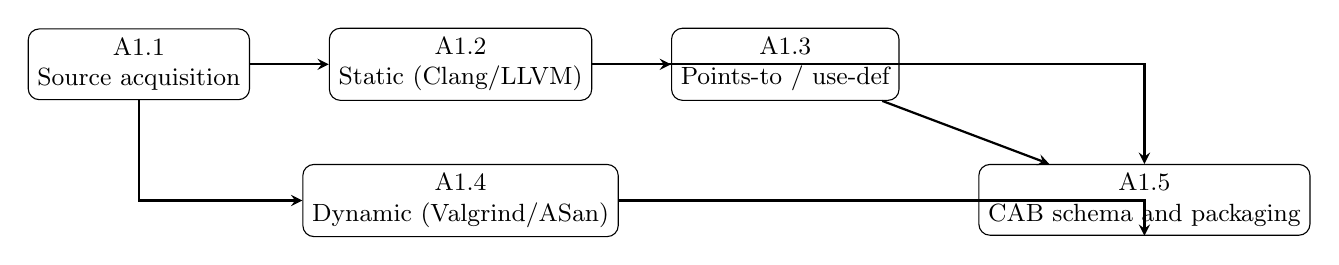
\begin{tikzpicture}[
    node distance=0.8cm and 1.0cm,
    box/.style={rectangle, draw, rounded corners, font=\small, align=center, minimum height=0.8cm},
    arrow/.style={->, >=stealth, thick}
]
\node[box] (a11) {A1.1\\Source acquisition};
\node[box, right=of a11] (a12) {A1.2\\Static (Clang/LLVM)};
\node[box, below=of a12] (a14) {A1.4\\Dynamic (Valgrind/ASan)};
\node[box, right=of a12] (a13) {A1.3\\Points-to / use-def};
\node[box, below right=of a13] (a15) {A1.5\\CAB schema and packaging};

\draw[arrow] (a11) -- (a12);
\draw[arrow] (a11) |- (a14);
\draw[arrow] (a12) -- (a13);
\draw[arrow] (a13) -- (a15);
\draw[arrow] (a14) -| (a15);
\draw[arrow] (a12) -| (a15);
\end{tikzpicture}
}
\caption{Dependency DAG of the analysis-phase sub-phases. A1.1 feeds A1.2 and A1.4; A1.3 consumes A1.2 outputs; A1.5 packages all outputs.}
\label{fig:dag}
\end{figure}

\subsection{Definition of done}
The Phase A deliverable is complete when all twenty-nine checkboxes are checked, the CAB validates against the schema, the function map covers every \libyaml{} function, and the pattern catalog identifies at least three concrete occurrences of every idiom I1--I10. The CAB is then handed to the OSG stage (Stage 2 of the Ferrous Bridge pipeline) for ownership-classification refinement and translation-engine input.

\begin{thebibliography}{99}

\bibitem{ferrousagent2026} M.~Long. The Ferrous Bridge Knowledge Base. Magneton Labs / YonedaAI Research Collective, April 2026.

\bibitem{c2rust2025} Galois and Immunant. \emph{c2rust: Migrate C99-compliant code to Rust}. \url{https://github.com/immunant/c2rust}, v0.21, October 2025.

\bibitem{ellison2012} C.~Ellison and G.~Ro\c{s}u. An executable formal semantics of C with applications. In \emph{POPL '12}, pages 533--544, 2012.

\bibitem{krebbers2015} R.~Krebbers. \emph{The C Standard Formalized in Coq}. PhD thesis, Radboud University, 2015.

\bibitem{memarian2019} K.~Memarian, V.~B.~F. Gomes, B.~Davis, S.~Kell, A.~Richardson, R.~N.~M. Watson, and P.~Sewell. Exploring C semantics and pointer provenance. \emph{Proc. ACM Program. Lang.}, 3(POPL):67:1--67:32, 2019.

\bibitem{leroy2009} X.~Leroy. Formal verification of a realistic compiler. \emph{Communications of the ACM}, 52(7):107--115, 2009.

\bibitem{zhang2023crown} H.~Zhang, C.~David, Y.~Yu, and M.~Wang. Ownership Guided C to Rust Translation. In \emph{CAV 2023}, pages 459--482, 2023.

\bibitem{emre2023laertes} M.~Emre, R.~Schroeder, K.~Dewey, and B.~Hardekopf. Translating C to Safer Rust. \emph{Proc. ACM Program. Lang.}, 5(OOPSLA):1--29, 2023.

\bibitem{sactor2025} \emph{SACTOR: LLM-Driven Correct and Idiomatic C to Rust Translation with Static Analysis and FFI-Based Verification}. Preprint, March 2025.

\bibitem{rustmap2025} \emph{RustMap: Dependency-Guided LLM C-to-Rust Translation}. Preprint, August 2025.

\bibitem{rustine2025} \emph{Rustine: Fully-Automated Repository-Level C-to-Rust Translation}. Preprint, October 2025.

\bibitem{orbit2026} \emph{ORBIT: Guided Agentic Orchestration for Autonomous C-to-Rust Transpilation}. Preprint, April 2026.

\bibitem{jung2026miri} R.~Jung et al. Miri: Practical Undefined Behavior Detection for Rust. In \emph{POPL 2026}, 2026.

\bibitem{kani2024} Amazon Web Services. \emph{Kani Rust Verifier}. \url{https://model-checking.github.io/kani/}, 2024.

\bibitem{jung2018rustbelt} R.~Jung, J.-H. Jourdan, R.~Krebbers, and D.~Dreyer. RustBelt: Securing the Foundations of the Rust Programming Language. \emph{Proc. ACM Program. Lang.}, 2(POPL):66:1--66:34, 2018.

\bibitem{landi1992undecidable} W.~Landi. Undecidability of static analysis. \emph{ACM Lett. Program. Lang. Syst.}, 1(4):323--337, 1992.

\bibitem{long2026c2rust} M.~Long. Compile-Time Supremacy: A Strategic Architecture for AI-Assisted C$\to$Rust Migration at Scale. GrokRxiv:2026.04.c2rust-compile-time-supremacy [cs.SE], April 2026.

\bibitem{rustpaper} M.~Long. Idiomatic Safe Rust for Streaming Parser Libraries: The \safelibyaml{} Target. GrokRxiv:2026.04.rust [cs.PL], April 2026 (forthcoming).

\bibitem{transpilingpaper} M.~Long. Automated C$\to$Rust Transpiling: Pipeline, Patterns, and Verification. GrokRxiv:2026.04.c-rust-transpiling [cs.PL], April 2026 (forthcoming).

\end{thebibliography}

\end{document}
